\documentclass[11pt,a4paper]{article}
\usepackage[utf8]{inputenc}
\usepackage[T1]{fontenc}
\usepackage[spanish,es-noshorthands]{babel}
\usepackage[margin=2.2cm]{geometry}
\usepackage{amsmath,amssymb}
\usepackage{graphicx}
\usepackage{booktabs}
\usepackage{longtable}
\usepackage{xcolor}
\usepackage{pdflscape}
\usepackage[colorlinks=true,linkcolor=blue!50!black,urlcolor=blue!50!black]{hyperref}
\setlength{\parskip}{5pt}
\setlength{\parindent}{0pt}
\newcommand{\dd}{\mathrm{d}}
\title{Dinámica de la pata con el robot apoyado\\
\large El caso que sirve para saber qué par pedirle al servo}
\author{Proyecto Segway con patas -- Robótica II, UNCUYO}
\date{\today}

\begin{document}
\maketitle

\section{Qué se plantea acá}

El robot está de pie sobre sus dos ruedas. El servo gira la manivela y, como la rueda apoya en el piso y no
se puede mover, lo que sube y baja es la cabina. Este es el caso que hay que resolver para saber qué par
necesita el servo: es el que tiene la masa de verdad, porque la cabina pesa casi cuatro veces más que la rueda.

Hay un solo grado de libertad, \(\theta\) (el ángulo del servo), y el camino es el de siempre: ángulos,
posiciones, velocidades, \(K\), \(U\), Lagrange. Lo que hay que mirar con cuidado es el paso de las
velocidades, porque ahí es donde entra que la rueda está quieta.

Se supone que el control de equilibrio mantiene el robot derecho mientras la pata se mueve, que las dos patas
se mueven juntas, y que la rueda no despega. Todo se escribe \textbf{por servo}: la energía del robot dividida
entre los dos.

\section{Las letras}

{\small\setlength{\tabcolsep}{5pt}
\begin{longtable}{l p{11.4cm}}
\toprule
\multicolumn{2}{l}{\textbf{La incógnita}}\\
\midrule
\(\theta\) & ángulo de la manivela \(AD\) por debajo de la horizontal. Es la coordenada generalizada, la única.
  \(10^\circ\) con la pata plegada, \(40^\circ\) estirada \\
\(\dot\theta,\;\ddot\theta\) & su velocidad y su aceleración, o sea cuán rápido y con qué aceleración gira el servo \\
\midrule
\multicolumn{2}{l}{\textbf{Las barras} (datos fijos del CAD)}\\
\midrule
\(AB\) & bancada, del eje del servo \(A\) al pivote \(B\). 80 mm, inclinada \(45^\circ\) \\
\(AD\) & manivela, la que mueve el servo. 112 mm \\
\(BC\) & balancín. 108 mm \\
\(CD\) & lado del acoplador que va a \(C\). 40.8 mm \\
\(DP\) & lado del acoplador que va al eje de la rueda \(P\). 112 mm \\
\(\delta\) & ángulo del acoplador en \(D\), entre \(DC\) y \(DP\). \(164^\circ\) \\
\(R_w\) & radio de la rueda. 33 mm \\
\midrule
\multicolumn{2}{l}{\textbf{Los ángulos que salen de \(\theta\)} (sección 3)}\\
\midrule
\(BD\) & diagonal del cuadrilátero, de \(B\) a \(D\). Cambia con \(\theta\) \\
\(\beta_1,\;\beta_2\) & ángulos en \(B\): \(\beta_1=\angle ABD\) y \(\beta_2=\angle DBC\) \\
\(\beta\) & ángulo interior del balancín en \(B\), \(\beta=\beta_1+\beta_2\) \\
\(\alpha_1,\;\alpha_2\) & ángulos en \(D\): \(\alpha_1=\angle ADB\) y \(\alpha_2=\angle BDC\) \\
\(\psi\) & giro del acoplador, medido desde la horizontal hasta la dirección \(D\!\to\!C\) \\
\(\beta',\;\psi'\) & cuánto giran el balancín y el acoplador por cada radián del servo: \(\beta'=\dd\beta/\dd\theta\),
  \(\psi'=\dd\psi/\dd\theta\) \\
\midrule
\multicolumn{2}{l}{\textbf{Las alturas} (sección 4)}\\
\midrule
\(y_P\) & altura del eje de la rueda \(P\) respecto de \(A\). Es negativa, porque \(P\) está abajo \\
\(y_P'\) & \(\dd y_P/\dd\theta\), cuánto baja \(P\) por cada radián del servo. También negativa \\
\(h\) & altura de la cabina sobre el piso, \(h=R_w-y_P\) \\
\midrule
\multicolumn{2}{l}{\textbf{Los coeficientes de velocidad} (sección 5)}\\
\midrule
\(c_Q\) & velocidad del punto \(Q\) por cada rad/s del servo, mirando desde la cabina. Es un vector, en m/rad \\
\(c_P\) & el de \(P\) (el eje de la rueda). El más grande de todos \\
\(c_{G_{AD}},\,c_{G_{BC}},\,c_{G_{CDP}}\) & los de los tres centros de masa \\
\(u\) & velocidad de la cabina por cada rad/s del servo, mirando desde el piso \\
\midrule
\multicolumn{2}{l}{\textbf{Las masas y las inercias}}\\
\midrule
\(m_{AD},\,m_{BC},\,m_{CDP}\) & masa de la manivela, del balancín y del acoplador. 23.2, 5.6 y 15.6 g \\
\(m_P\) & rueda más motor, que cuelgan de \(P\). 182 g \\
\(m_c\) & masa de la cabina, o sea todo lo que no es pata. 667 g \\
\(n\) & cantidad de patas. 2 \\
\(I_{AD},\,I_{BC},\,I_{CDP}\) & inercia de cada pieza respecto de \emph{su propio} centro de masa \\
\midrule
\multicolumn{2}{l}{\textbf{Lo que entra desde afuera}}\\
\midrule
\(\tau\) & par del servo sobre su manivela, positivo en el sentido en que crece \(\theta\) \\
\(b_A,b_B,b_C,b_D\) & fricción viscosa en cada articulación (sección 8) \\
\(g\) & gravedad \\
\bottomrule
\end{longtable}}

\section{Paso 1: los ángulos en función de \(\theta\)}

Todo el mecanismo queda definido por \(\theta\). Los ángulos se sacan con la ley del coseno, apoyándose en la
diagonal \(BD\), que parte el cuadrilátero en dos triángulos: \(ABD\) y \(BDC\). La figura de la página
siguiente los muestra todos.

Primero la diagonal, con el triángulo \(ABD\), donde el ángulo en \(A\) vale \(\theta+45^\circ\):
\begin{equation}
BD=\sqrt{AB^2+AD^2-2\,AB\,AD\cos(\theta+45^\circ)} .
\label{eq:BD}
\end{equation}
Con \(BD\) ya conocida, los dos triángulos quedan con los tres lados conocidos, así que todos sus ángulos
salen por ley del coseno:
\begin{align}
\beta_1&=\cos^{-1}\!\left(\frac{AD^2-AB^2-BD^2}{-2\,AB\,BD}\right), &
\beta_2&=\cos^{-1}\!\left(\frac{CD^2-BC^2-BD^2}{-2\,BC\,BD}\right), \label{eq:beta}\\
\alpha_1&=\cos^{-1}\!\left(\frac{AB^2-BD^2-AD^2}{-2\,BD\,AD}\right), &
\alpha_2&=\cos^{-1}\!\left(\frac{BC^2-BD^2-CD^2}{-2\,BD\,CD}\right), \label{eq:alfa}
\end{align}
y de ahí el ángulo del balancín y el giro del acoplador:
\begin{equation}
\beta=\beta_1+\beta_2,\qquad\qquad \boxed{\;\psi=180^\circ-\theta-\alpha_1-\alpha_2\;}
\label{eq:psi}
\end{equation}
La segunda sale de mirar el punto \(D\): la dirección \(D\!\to\!A\) forma \(180^\circ-\theta\) con la
horizontal, y desde ahí hay que girar \(\alpha_1\) para llegar a \(D\!\to\!B\) y \(\alpha_2\) más para llegar a
\(D\!\to\!C\).

Las derivadas \(\beta'\) y \(\psi'\) (cuánto gira cada barra por radián del servo) salen de derivar
\eqref{eq:beta} a \eqref{eq:psi}; la cuenta está hecha en \texttt{dinamica\_resumen.pdf} y el resultado es
\begin{equation}
\beta'=-\bigl(\cot\alpha_1+\cot\alpha_2\bigr)\frac{AB\,AD\sin(\theta+45^\circ)}{BD^2},\qquad
\psi'=-1+\bigl(\cot\beta_1+\cot\beta_2\bigr)\frac{AB\,AD\sin(\theta+45^\circ)}{BD^2}.
\label{eq:derivadas}
\end{equation}

\textbf{De acá en adelante no se vuelve a tocar la geometría.} Todo lo que sigue usa \(\beta\), \(\psi\),
\(\beta'\) y \(\psi'\) como números que ya están calculados para cada \(\theta\).

\begin{landscape}
\vspace*{\fill}
\begin{center}

\includegraphics[width=\linewidth]{fig_dinamica.png}
\end{center}
\vspace*{\fill}
\end{landscape}

\section{Paso 2: las alturas}

Con los ángulos ya resueltos, las posiciones son trigonometría directa. La que importa para todo lo que sigue
es la del eje de la rueda:
\begin{equation}
y_P(\theta)=-AD\sin\theta+DP\sin(\psi+\delta),
\label{eq:yP}
\end{equation}
que es negativa porque \(P\) está por debajo de \(A\).

Y acá viene lo propio del robot apoyado. Como la rueda toca el piso, su eje \(P\) queda siempre a la altura
\(R_w\), no importa qué haga el servo. Entonces, si \(A\) está a una altura \(Y_A\) y \(P\) está \(y_P\) por
debajo de \(A\), la condición de apoyo \(Y_A+y_P=R_w\) da
\begin{equation}
\boxed{\;h(\theta)=R_w-y_P(\theta)\;}
\label{eq:h}
\end{equation}
La altura de la cabina es una función de \(\theta\). No hay una coordenada nueva: mover el servo es subir y
bajar la cabina, y \(y_P\) (que ya venía de la cinemática) es el que dice cuánto. El panel (a) de la figura de
la página siguiente lo muestra.

\section{Paso 3: las velocidades}

\textbf{Primero, desde la cabina.} Para cada punto \(Q\) del mecanismo se define \(c_Q\), su velocidad por
cada rad/s del servo, medida parándose sobre la cabina:
\begin{equation}
\mathbf{v}^{\,\text{cabina}}_Q=c_Q(\theta)\,\dot\theta .
\label{eq:cQ}
\end{equation}
Son vectores que se calculan de una vez con los ángulos del paso 1. Con \(\mathbf{k}\times(x,y)=(-y,x)\):
\begin{align}
c_{G_{AD}}&=-\,\mathbf{k}\times G_{AD}, & &\text{la manivela gira alrededor de } A \text{ a } -\dot\theta; \label{eq:cAD}\\
c_{G_{BC}}&=\beta'\,\mathbf{k}\times(G_{BC}-B), & &\text{el balancín gira alrededor de } B \text{ a } \beta'\dot\theta; \label{eq:cBC}\\
c_Q&=c_D+\psi'\,\mathbf{k}\times(Q-D), & &\text{el acoplador, para } Q=P \text{ o } Q=G_{CDP}. \label{eq:cCDP}
\end{align}
El más grande es \(c_P\) (el del eje de la rueda): en \(\theta=25^\circ\) mide 199 mm/rad, o sea que por cada
radián que gira el servo la rueda se aleja 199 mm de la cabina. Panel (b) de la figura.

\textbf{Ahora, desde el piso.} Llamamos \(u\) a la velocidad de la cabina por cada rad/s del servo. Como la
cabina solo se traslada, la velocidad de cualquier punto \(Q\) de la pata vista desde el piso es la de la
cabina más la que tenía respecto de ella:
\begin{equation}
\mathbf{v}_Q=\bigl(u+c_Q\bigr)\dot\theta .
\label{eq:vpiso}
\end{equation}
La rueda está quieta, o sea \(\mathbf{v}_P=0\), y de ahí sale \(u\):
\begin{equation}
\boxed{\;u=-c_P\;}
\label{eq:u}
\end{equation}
Es el mismo vector cambiado de signo: lo que la rueda bajaba respecto de la cabina, ahora lo sube la cabina
respecto del piso. Con eso, todas las velocidades quedan:
\begin{center}\small
\begin{tabular}{ll}
\toprule
la cabina & \(-c_P\,\dot\theta\) \quad (sube) \\
la rueda y el motor, en \(P\) & \(0\) \quad (están quietos) \\
cada centro de masa \(G\) de la pata & \(\bigl(c_G-c_P\bigr)\dot\theta\) \\
\bottomrule
\end{tabular}
\end{center}
Panel (c) de la figura. Las velocidades angulares no cambian, porque la cabina no gira: la manivela sigue a
\(-\dot\theta\), el balancín a \(\beta'\dot\theta\) y el acoplador a \(\psi'\dot\theta\).

\begin{landscape}
\vspace*{\fill}
\begin{center}
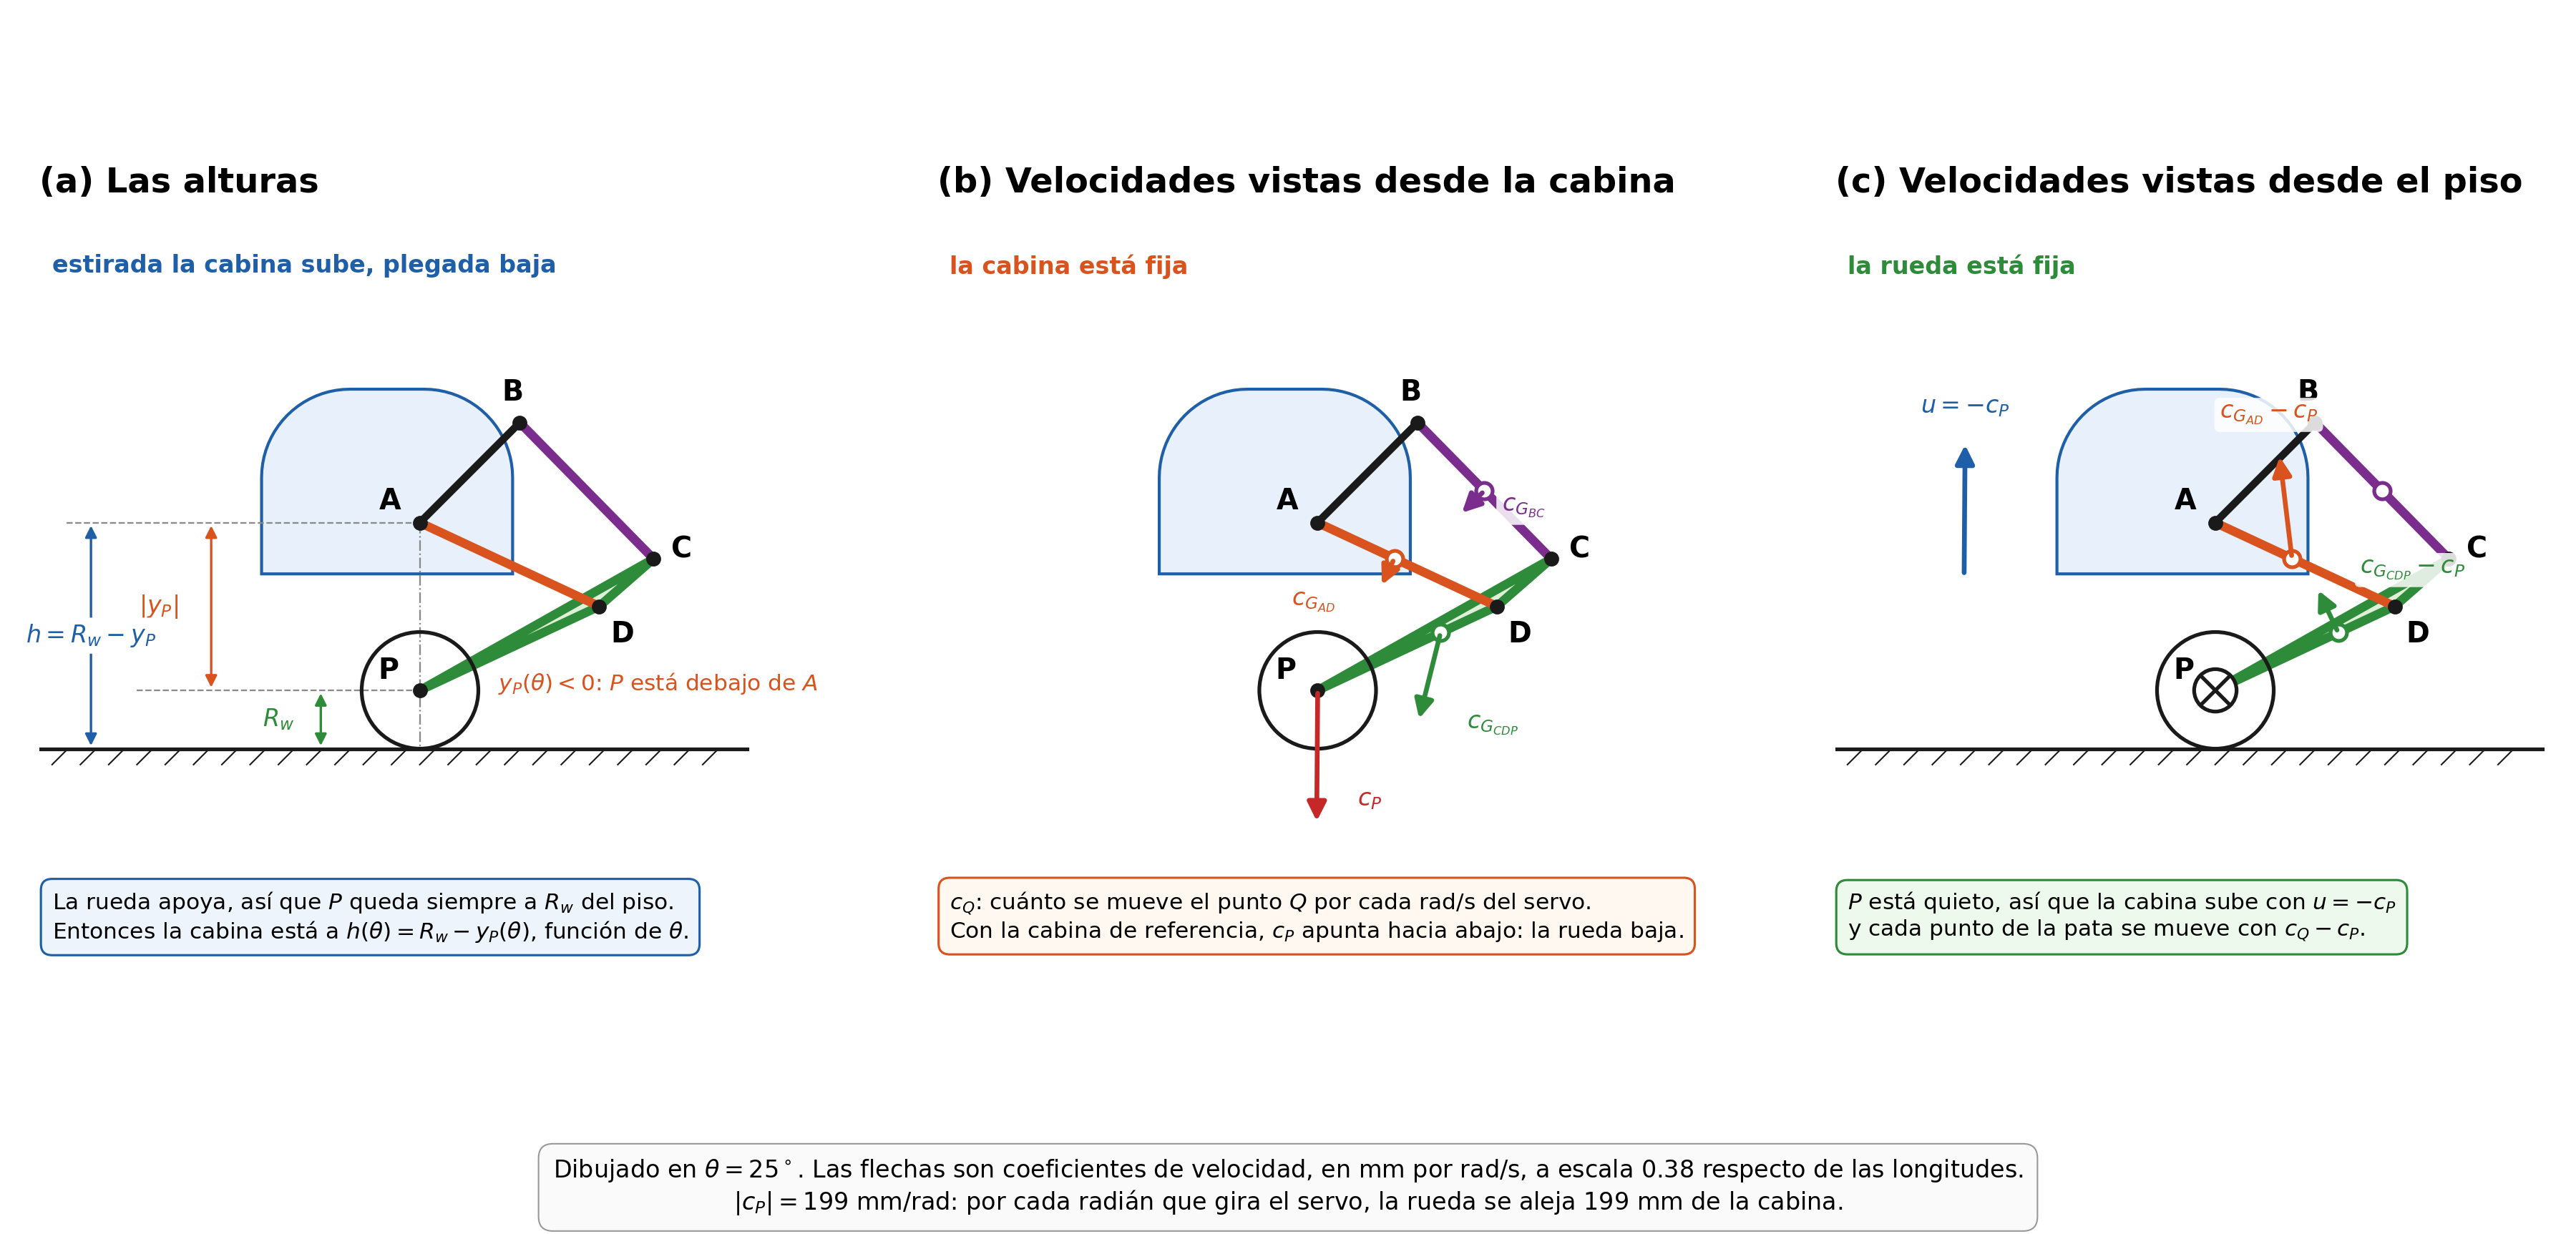
\includegraphics[width=\linewidth]{fig_apoyado.png}
\end{center}
\vspace*{\fill}
\end{landscape}

\section{Paso 4: la energía cinética \(K\)}

Cada cuerpo aporta la traslación de su centro de masa más su giro propio. Poniendo las velocidades del paso 3:
\begin{equation}
\begin{aligned}
K={}&\tfrac12\,m_{AD}\bigl|c_{G_{AD}}-c_P\bigr|^2\dot\theta^2 \;+\; \tfrac12\,I_{AD}\,\dot\theta^2
  &&\text{manivela: traslada y gira}\\
+{}&\tfrac12\,m_{BC}\bigl|c_{G_{BC}}-c_P\bigr|^2\dot\theta^2 \;+\; \tfrac12\,I_{BC}\,\beta'^2\dot\theta^2
  &&\text{balancín: traslada y gira a }\beta'\dot\theta\\
+{}&\tfrac12\,m_{CDP}\bigl|c_{G_{CDP}}-c_P\bigr|^2\dot\theta^2 \;+\; \tfrac12\,I_{CDP}\,\psi'^2\dot\theta^2
  &&\text{acoplador: traslada y gira a }\psi'\dot\theta\\
+{}&\;0
  &&\text{rueda y motor: están quietos}\\
+{}&\tfrac12\,\frac{m_c}{n}\bigl|c_P\bigr|^2\dot\theta^2
  &&\text{la cabina, que sube y baja}
\end{aligned}
\label{eq:K}
\end{equation}
Todos los términos tienen \(\dot\theta^2\) de factor común, así que
\begin{equation}
K=\tfrac12\,I_{eq}(\theta)\,\dot\theta^2,
\label{eq:KIeq}
\end{equation}
\begin{equation}
\boxed{\;
\begin{aligned}
I_{eq}(\theta)={}&I_{AD}+I_{BC}\,\beta'^2+I_{CDP}\,\psi'^2\\
&+m_{AD}\bigl|c_{G_{AD}}-c_P\bigr|^2+m_{BC}\bigl|c_{G_{BC}}-c_P\bigr|^2+m_{CDP}\bigl|c_{G_{CDP}}-c_P\bigr|^2\\
&+\frac{m_c}{n}\bigl|c_P\bigr|^2
\end{aligned}
\;}
\label{eq:Ieq}
\end{equation}
\(I_{eq}\) (la inercia equivalente) es lo que el servo siente en su eje. Depende de \(\theta\) porque las
relaciones de transmisión \(\beta'\) y \(\psi'\) y el vector \(c_P\) cambian con la posición. El último
término, el de la cabina, es el 93 por ciento del total.

\section{Paso 5: la energía potencial \(U\)}

Solo gravedad, con las alturas medidas desde el piso:
\begin{equation}
U=g\left[\frac{m_c}{n}\,\underbrace{(R_w-y_P)}_{\text{cabina}}
+m_{AD}\,h_{G_{AD}}+m_{BC}\,h_{G_{BC}}+m_{CDP}\,h_{G_{CDP}}
+m_P\,\underbrace{R_w}_{\text{constante}}\right],
\label{eq:U}
\end{equation}
donde la altura de cada centro de masa de la pata es \(h_G=R_w+(y_G-y_P)\), es decir la del eje de la rueda
más lo que ese punto esté por encima de \(P\).

Dos cosas para notar. La cabina entra con \(R_w-y_P\), que es \eqref{eq:h}, y es el término que manda. Y la
rueda entra con \(R_w\), que es constante: al derivar desaparece, porque la rueda no sube ni baja.

La derivada sale directo, porque la velocidad vertical de cada punto por unidad de \(\dot\theta\) es la segunda
componente de su vector de velocidad:
\begin{equation}
\boxed{\;
U'(\theta)=g\left[\frac{m_c}{n}\bigl(-c_{P,y}\bigr)
+m_{AD}\bigl(c_{G_{AD},y}-c_{P,y}\bigr)+m_{BC}\bigl(c_{G_{BC},y}-c_{P,y}\bigr)+m_{CDP}\bigl(c_{G_{CDP},y}-c_{P,y}\bigr)\right]
\;}
\label{eq:dU}
\end{equation}
con \(c_{Q,y}\) la componente vertical de \(c_Q\). Como \(c_{P,y}\) es negativa, el primer término es positivo:
\(U\) crece con \(\theta\), o sea que estirar la pata es levantar el robot, y por eso el peso siempre tiende a
plegarla.

\section{Paso 6: lo que no sale de \(K\) ni de \(U\)}

Quedan dos cosas: el par del servo y la fricción. Las dos entran por su trabajo virtual, no por el
lagrangiano.

\textbf{El par del servo.} \(\tau\) actúa directamente sobre \(\theta\), así que su fuerza generalizada es
\(\tau\) sin ningún factor. Es la incógnita que buscamos.

\textbf{La fricción.} Hay una articulación en cada esquina del cuadrilátero, y en cada una hay roce
proporcional a la velocidad angular \emph{relativa} entre las dos piezas que une. Con las velocidades
angulares del paso 3 (la cabina quieta, la manivela a \(-\dot\theta\), el balancín a \(\beta'\dot\theta\) y el
acoplador a \(\psi'\dot\theta\)), esas velocidades relativas son:
\begin{center}\small
\begin{tabular}{llll}
\toprule
Articulación & Une & Velocidad relativa & En \(\theta=25^\circ\) \\
\midrule
\(A\) & cabina con manivela (es el eje del servo) & \(-\dot\theta\) & \(1.00\,\dot\theta\) \\
\(B\) & cabina con balancín & \(\beta'\dot\theta\) & \(0.95\,\dot\theta\) \\
\(C\) & balancín con acoplador & \((\psi'-\beta')\,\dot\theta\) & \(1.91\,\dot\theta\) \\
\(D\) & manivela con acoplador & \((\psi'+1)\,\dot\theta\) & \(1.96\,\dot\theta\) \\
\bottomrule
\end{tabular}
\end{center}
La función de disipación de Rayleigh junta las cuatro,
\(D=\tfrac12\bigl[b_A\dot\theta^2+b_B(\beta'\dot\theta)^2+b_C((\psi'-\beta')\dot\theta)^2+b_D((\psi'+1)\dot\theta)^2\bigr]\),
y el par de roce que ve el servo es \(-\partial D/\partial\dot\theta=-b_{eq}(\theta)\,\dot\theta\), con
\begin{equation}
\boxed{\;b_{eq}(\theta)=b_A+b_B\,\beta'^2+b_C\,(\psi'-\beta')^2+b_D\,(\psi'+1)^2\;}
\label{eq:beq}
\end{equation}
Tiene la misma forma que \(I_{eq}\): cada articulación entra con el cuadrado de su relación de transmisión.
Las que más rozan son \(C\) y \(D\), que giran casi el doble que el servo.

\textbf{Atención: hoy los cuatro valen cero.} No están medidos, así que el modelo no tiene ninguna pérdida y
por eso es optimista en las simulaciones rápidas. \(b_A\) es el más importante de los cuatro, porque incluye
la reductora del propio servo. Para medir \(b_{eq}\): dejar el servo libre, soltar la pata desde estirada y
cronometrar cuánto tarda en plegarse; se ajusta \(b_A\) hasta que la simulación tarde lo mismo. Si al medir
aparece un par de arranque que no depende de la velocidad, es fricción seca y se agrega como
\(-\operatorname{sign}(\dot\theta)\bigl[c_A+c_B|\beta'|+c_C|\psi'-\beta'|+c_D|\psi'+1|\bigr]\).

\textbf{Lo que no aparece.} La reacción del piso \(N\) no está en ninguna parte. El punto de contacto no se
mueve, así que no hace trabajo, y el peso que soporta ya está contado dentro de \(U\).

\section{Paso 7: la ecuación}

Con \(L=K-U\), y usando que \(K=\tfrac12 I_{eq}(\theta)\dot\theta^2\) depende de \(\theta\) además de
\(\dot\theta\):
\begin{equation}
\frac{\partial L}{\partial\dot\theta}=I_{eq}\,\dot\theta,\qquad
\frac{\dd}{\dd t}\frac{\partial L}{\partial\dot\theta}=I_{eq}\,\ddot\theta+I_{eq}'\,\dot\theta^2,\qquad
\frac{\partial L}{\partial\theta}=\tfrac12\,I_{eq}'\,\dot\theta^2-U',
\label{eq:parciales}
\end{equation}
donde \(I_{eq}'=\dd I_{eq}/\dd\theta\). Restando y poniendo las fuerzas del paso 6 del lado derecho:
\begin{equation}
\boxed{\;
I_{eq}(\theta)\,\ddot\theta\;+\;\tfrac12\,I_{eq}'(\theta)\,\dot\theta^2\;+\;U'(\theta)
\;=\;\tau\;-\;b_{eq}(\theta)\,\dot\theta
\;}
\label{eq:final}
\end{equation}
Leída de izquierda a derecha: para mover la pata el servo tiene que vencer la inercia, un término extra que
aparece porque esa inercia cambia con la posición, el peso, y el roce.

Los dos casos que más se usan salen de acá. Con la pata quieta (\(\dot\theta=\ddot\theta=0\)), el par para
sostenerla es
\begin{equation}
\tau_{est}(\theta)=U'(\theta).
\label{eq:tauest}
\end{equation}
Y para simular, despejando la aceleración, con el estado \(x=(\theta,\dot\theta)\):
\begin{equation}
\ddot\theta=\frac{\tau-b_{eq}\,\dot\theta-\tfrac12 I_{eq}'\,\dot\theta^2-U'}{I_{eq}} .
\label{eq:estado}
\end{equation}

\section{Resumen: qué términos aparecieron}

\begin{center}\small
\begin{tabular}{l p{10.6cm}}
\toprule
\textbf{En \(K\)} & \\
\midrule
Entró la cabina & \(\tfrac12(m_c/n)|c_P|^2\dot\theta^2\). Es el término más grande, el 93 por ciento de
  \(I_{eq}\). No estás subiendo la rueda, estás subiendo la cabina \\
Salió la rueda & el término de \(m_P\) desaparece: con la rueda apoyada, \(P\) no se traslada \\
Cambió la referencia & las velocidades pasan de \(c_Q\) a \(c_Q-c_P\): todo se mide respecto de \(P\) \\
Salió el giro de la rueda & \(\tfrac12 I_P\omega^2\) no depende de \(\theta\), lo impone el motor de tracción \\
\midrule
\textbf{En \(U\)} & \\
\midrule
Entró la cabina & \((m_c/n)\,g\,(R_w-y_P)\), otra vez el término que manda \\
Salió la rueda & su altura es \(R_w\), constante, y al derivar se va \\
\midrule
\textbf{Fuera de \(K\) y \(U\)} & \\
\midrule
El par del servo & \(\tau\), que entra directo sobre \(\theta\) \\
La fricción & \(-b_{eq}(\theta)\,\dot\theta\), con las cuatro articulaciones pesadas por el cuadrado de su
  relación de transmisión. Hoy vale cero por falta de medición \\
No aparece \(N\) & el contacto no se mueve, no hace trabajo \\
\midrule
\textbf{En la ecuación} & \\
\midrule
\(\tfrac12 I_{eq}'\dot\theta^2\) & aparece porque \(I_{eq}\) cambia con \(\theta\). Es el equivalente al
  término centrífugo de un mecanismo de inercia variable \\
\bottomrule
\end{tabular}
\end{center}

\section{Números}

Con los valores de la tabla de la sección 2, y \(n=2\):

\begin{center}\small
\begin{tabular}{lrrr}
\toprule
 & \(\theta=10^\circ\) (plegada) & \(\theta=25^\circ\) & \(\theta=40^\circ\) (estirada) \\
\midrule
Altura de la cabina \(h\) [mm] & 70.2 & 127.9 & 177.2 \\
\(\beta'\), \(\psi'\) [rad/rad] & \(-0.703\), \(1.260\) & \(-0.950\), \(0.964\) & \(-1.161\), \(1.120\) \\
\(|c_P|=|y_P'|\) [mm/rad] & 250 & 199 & 182 \\
\(I_{eq}\) [g\,m\(^2\)] & 22.24 & 14.13 & 11.92 \\
\(\tau_{est}=U'\) [kg\,cm] & 9.06 & 7.20 & 6.58 \\
\midrule
Factor de \(b_C\) en \(b_{eq}\) & 3.85 & 3.66 & 5.20 \\
Factor de \(b_D\) en \(b_{eq}\) & 5.11 & 3.86 & 4.49 \\
\bottomrule
\end{tabular}
\end{center}

La postura más exigente es la plegada: ahí el brazo \(|c_P|\) es máximo y el servo tiene que dar 9.1 kg\,cm
solo para sostener el robot quieto, contra los 40 kg\,cm del servo elegido. La inercia también es máxima ahí, casi
el doble que estirada.

\section{Qué no incluye este modelo}

Supone que la cabina no gira, es decir que el control de equilibrio la mantiene derecha mientras la pata se
mueve, y que las dos patas van juntas. No dice nada sobre el equilibrio en sí ni sobre el avance: para eso
hace falta el modelo de tres grados de libertad \((x,\varphi,\theta)\), que es el paso siguiente y que
reutiliza todo lo de las secciones 3 a 5.

Tampoco vale mientras el robot está en el aire, porque ahí la rueda no está quieta y \(u\) es otro. Ese caso,
y el de la pata en un banco con la cabina amurada, están en \texttt{dinamica\_resumen.pdf} junto con el
cálculo de la caída de un escalón.

Las masas y las inercias son estimaciones (la primera iteración del CAD escalada a 80, y las fichas del motor y del servo), y las cuatro fricciones son cero. Los dos pendientes de
medición son pesar las piezas impresas y hacer el ensayo de caída libre de la pata.

\section{Archivos}

\begin{itemize}
\item \texttt{dinamica\_pata.m}: sección 1 los parámetros, para editar; sección 2 los tres casos; sección 3 una
  simulación de agacharse y pararse; sección 4 la verificación contra los diagramas de cuerpo libre; sección 5
  la caída de un escalón; sección 6 la fuerza radial en el eje del servo. El caso de este documento se elige con la cadena \texttt{'parado'}.
\item \texttt{fig\_dinamica.py} \(\to\) \texttt{fig\_dinamica.png}: los ángulos de la sección 3.
\item \texttt{fig\_apoyado.py} \(\to\) \texttt{fig\_apoyado.png}: las alturas y los coeficientes de velocidad.
\item \texttt{../cinematica/parametros\_geometria.m}: la geometría, misma fuente para todo el proyecto.
\end{itemize}

\end{document}
